\chapter{Some Vectorial Finite Elements}\label{aux_label43}
\section*{Introducci\'on al cap\'itulo}
Los elementos $H(\Div)$--conformes fueron definidos 
para construir un operador de interpolaci\'on natural 
para campos vectoriales con componentes normales conti\-nuas.
An\'alogamente, los otros elementos considerados son 
conformes en $H(\bcurl)$, que son usados para interpolar campos
vectoriales con componentes tangenciales continuas. Estos son los casos
de las soluciones de las ecuaciones de Maxwell arm\'onicas en el
tiempo~\cite{monk}, y de la formulaci\'on mixta del 
problema de Poisson~\cite{boffiBrezziFortin}.

A pesar de poner la construcci\'on y explicitar
algunas propiedades para ambas clases de elementos
aqu\'i, dejamos las estimaciones
que demostramos para el caso $H(\bcurl)$ para el 
Cap\'itulo~\ref{auxlabel202}, pues no ser\'an usadas en la aplicaci\'on
final (Cap\'itulo~\ref{auxLabel100}).

Adoptaremos la convenci\'on de que
los objetos como funciones, variables, vectores normales 
en el Prisma de referencia
$\hat{E}$ tendr\'an un sombrero como $\hat{\bu}, \hat{\bx}, \hat{\bn},\ldots$
al mismo tiempo que el sombrero denotar\'a una transformaci\'on
de \emph{pullback} correspondiente a una aplicaci\'on de
$\hat{E}$ hacia un elemento f\'isico $E$.

%As we are going to deal with vectorial Finite Elements and
%vectorial Virtual Elements, we are going to need to use the following notational convention.
%\begin{notation} If\hspace{5pt}$V$ denotes a functional space of vectorial
%fields in $\mathbb{R}^n$, whether finite dimensional
%or not, $(V)_i$ denotes the space of scalar functions in the $i-$th
%coordinate projection
%of $V$, for $1\leqslant i\leqslant n$.
%\end{notation}
Para los espacios de funciones polinomiales de tipo producto tensorial
involucrados en la construcci\'on de los elementos 
$H(\bcurl)$--conformes o $H(\Div)$--conformes 
requeriremos de la siguiente notaci\'on.
\begin{notacion}\label{auxlabel208}
Polinomios definidos en un prisma:
  \begin{IEEEeqnarray*}{rCl}
    P_{k,l} 	&:=& P_k(\hat x_1,\hat x_2) 	 \otimes P_{l}(\hat x_3)\mbox{,} \\
    Q_{k,l,m} 	&:=& P_k(\hat{x}_1) \otimes P_l(\hat{x}_2)\otimes P_m(\hat{x}_3).
  \end{IEEEeqnarray*}
Dada una cara $f$ de un elemento poliedral, en la cual tenemos variables 
locales $(\xi_1,\xi_2)$, el espacio $Q_{k,l}$ ser\'a definido como
  \begin{IEEEeqnarray*}{rCl}
  	Q_{k,l} &=&	P_{k}(\xi_1) \otimes P_l(\xi_2).
  \end{IEEEeqnarray*}
\end{notacion}
\section*{Introduction to the chapter}
$H(\Div)$--conforming elements were
defined to determine a natural interpolation operator for fields with continuous normal components.
Similarly, the other elements considered are $H(\bcurl)$--conforming, which are used 
to interpolate fields with continuous tangential components. These two are the cases of the
solutions of time harmonic Maxwell's equations, and the
solution of the mixed formulation of the Poisson problem.
Although we put the construction and state some properties for both
kinds of elements here, we leave the estimates proved for the $H(\bcurl)$ case
for Chapter~\ref{auxlabel202}, as they are not used in the main application
in Chapter~\ref{auxLabel100}.

We will adopt the convention that objects like functions, variables, normals 
in the reference
prism $\hat{E}$ will have a hat as in $\hat{\bu}, \hat{\bx}, \hat{\bn},\ldots$
and then also the hat will denote a pullback transformation corresponding
to a mapping from $\hat{E}$ onto  a physical element $E$.

%As we are going to deal with vectorial Finite Elements and
%vectorial Virtual Elements, we are going to need to use the following notational convention.
%\begin{notation} If\hspace{5pt}$V$ denotes a functional space of vectorial
%fields in $\mathbb{R}^n$, whether finite dimensional
%or not, $(V)_i$ denotes the space of scalar functions in the $i-$th
%coordinate projection
%of $V$, for $1\leqslant i\leqslant n$.
%\end{notation}
For tensor product polynomial spaces involved in the construction
of $H(\bcurl)$ or $H(\Div)$ elements we will need the following notation.
\begin{notation}\label{auxlabel200}
For polynomials defined over polyhedra we add the following symbols:
  \begin{IEEEeqnarray*}{rCl}
    P_{k,l} 		&:=& P_{k}(\hat x_1,\hat x_2) 	 \otimes P_{l}(\hat x_3)\mbox{,} \\
    Q_{k,l,m} 	&:=& P_k(\hat{x}_1) \otimes P_l(\hat{x}_2)\otimes P_m(\hat{x}_3)\mbox{,}
  \end{IEEEeqnarray*}
  and for a given face $f$ on a polyhedron, in which we have local variables 
  $(\xi_1,\xi_2)$, the space $Q_{k,l}$ will be defined as
  \begin{IEEEeqnarray*}{rCl}
  	Q_{k,l} &=&	P_{k}(\xi_1) \otimes P_l(\xi_2).
  \end{IEEEeqnarray*}
\end{notation}
%=============================================================
%\noindent---------------------------------------------------------
%% h div low order reference prism
\paragraph{$k=1$} (lowest order basis elements)\\[5pt] % (fold)
\label{par:_k_0_}
\begin{IEEEeqnarraybox*}{rCl}
	v_1&=&\left(
		\begin{array}{c}
			-1+x_1\\
			x_2\\[3pt]
			0\\
		\end{array}
	\right)
\end{IEEEeqnarraybox*}
\begin{IEEEeqnarraybox*}{rCl}
	v_2&=&\left(
		\begin{array}{c}
			x_1\\
			-1+x_2\\[3pt]
			0\\
		\end{array}
	\right)
\end{IEEEeqnarraybox*}
% paragraph _k_0_ (end)\\
%---------------------------------------------------------
%=============================================================
\section{Prismatic Finite Elements}
%>this intends to be an extension of the treatment
%in~\cite{giraultRaviart} to prismatic elements?
\subsection{$H(\bcurl)$--Conforming Element on Prisms} % (fold)
\label{sub:defEdgeElement}
First we introduce two more polynomial spaces on the reference prism of
Figure~\ref{reference_prism}.
$\hat{T}$ denotes the triangle in Definition~\ref{defi_of_ref_prism} and 
$\hat I = [0,1]$.
\begin{defi} For an integer $k\geqslant 1$, let $R_k(\hat{T})$ denote the space of polynomials, defined over the
triangle $\hat{T}$, given by
\begin{IEEEeqnarray}{rCl}
    \label{defRk}
    R_k(\hat{T}) & := & P_{k-1}(\hat{T})^2 \oplus S_k(\hat{T})
\end{IEEEeqnarray}
where
\begin{IEEEeqnarray}{rClCrCl}
    \label{defSk}
    S_k(\hat{T}) & := & \{ \bp\in \widetilde{P}_k^2 \,:\;\bp\cdot\hat\bx =
    0\}\mbox{,}\quad\hat\bx & = & (\hat x_1, \hat x_2)'.
\end{IEEEeqnarray}
\end{defi}
\facesOfPrism
\edgesOfPrism
\begin{figure}[!h]
  \centering
  \subfloat
  {
    \label{unitTanPrism}
    \unitTangentsPrism
  }
  \caption{Directions of positive unit tangents (cfr. Table~\ref{prismNotationTableEdges}).}
\end{figure}
\begin{defi}\label{edgeelement} Given a natural $k$, the $H(\bcurl)$--Conforming 
Finite Element of degree $k$ is defined by the following triple.
\begin{enumerate}
  \item $\hat{E}$ is the reference prism in Definition~\ref{defi_of_ref_prism}.
  \item The polynomial space $P_{\hat{E}}$ is
        \begin{IEEEeqnarray}{rCl} \label{spaceFEprismHcurl}
            P_{\hat{E}} & = & R_k(\hat{T}) \otimes P_k(\hat{I}) \times 
            P_k(\hat{T}) \otimes P_{k-1}(\hat{I}).
         \end{IEEEeqnarray} 
  \item The degrees of freedom are (cfr. Tables~\ref{prismNotationTableFaces} 
and~\ref{prismNotationTableEdges}):
  {\color{Orange} ver si en~\ref{momentos2hcurl} y los otros de caras
    hay que cambiar orden de componentes o signos por lo que acomod'e para definir el elemento
    af'in; ver~(\ref{momentos2hcurlPhys})}.
\begin{IEEEeqnarray}{ll}
    \label{momentos1hcurl}  
    \hat\varphi_{\hat{\be},\hat{q}}\,(\hat\bu) = 
    \int_{\hat\be} \hat q\,\hat\bu\cdot d\hat\balpha\mbox{,}  
      & \hat q\in P_{k-1}(\hat\be)\mbox{, for each edge $\hat\be$;}\\[8pt]%with unit tangent } \boldsymbol{\tau} \mbox{;}}
    \nonumber\hat\varphi_{\hat f,\hat\bq}\,(\hat\bu) =  
    \int_{\hat f} \hat\bu \times \hat\bn \cdot \hat\bq\,
    d\hat S\mbox{, }\quad&\hat\bq = (\hat q_1,\hat q_2,0) \in P_{k-2}^2 \times \{ 0 \},\\[4pt] 
    \label{momentos2hcurl} 
      &\mbox{ for each face $f=\hat f_3$ or$\hat f_4$;}\\[8pt]
    \nonumber\hat\varphi_{\hat f_1,\hat\bq}\,(\hat\bu) =  
    \int_{\hat f_1} \hat\bu \times \hat\bn_1 \cdot \hat\bq\,
    d\hat S\mbox{, }\quad&
      \hat\bq = (0,\hat q_3,\hat q_2)\mbox{, }\hat q_3\in Q_{k-2,k-1}\mbox{,}\\[4pt]
    \label{momentos3hcurl}
      &\hat q_2 \in Q_{k-1,k-2}\mbox{;}\\[8pt]   %\mbox{, for the face } \hat f_1
    \nonumber\hat\varphi_{\hat f_2,\hat\bq}\,(\hat\bu) =  
    \int_{\hat f_2} \hat\bu \times \hat\bn_2 \cdot \hat\bq\,
    d\hat S\mbox{, }\quad& 
      \hat\bq = (\hat q_3,0,\hat q_1)\mbox{, }\hat q_3 \in Q_{k-2,k-1}\mbox{,}\\[4pt]
    \label{momentos4hcurl}
      &\hat q_1 \in Q_{k-1,k-2}\mbox{;}\\[8pt]   %\mbox{, for the face } \hat f_2
    \nonumber\hat\varphi_{\hat f_5,\hat\bq}\,(\hat\bu) =  
    \int_{\hat f_5} \hat\bu \times \hat\bn_5 \cdot \hat\bq\,
    d\hat S\mbox{, }\quad&
      \hat\bq = (0,\hat q_3,\hat q_1)\mbox{, }\hat q_3 \in Q_{k-2,k-1}\mbox{,}\\[4pt]
    \label{momentos5hcurl}
      &\hat q_1 \in Q_{k-1,k-2}\mbox{;}\\[8pt]   %\mbox{, for the face } \hat f_5
    \nonumber\hat\varphi_{\hat\br}\,(\hat\bu) = 
    \int_{\hat{E}} \hat\bu \cdot \hat\br \, d\hat\bx\mbox{, }&\hat r_1\mbox{, } 
    \hat r_2 \in P_{k-2,k-2}\mbox{, }\\[4pt]
    \label{momentos6hcurl}
      &\hat r_3 \in P_{k-3,k-1}.
\end{IEEEeqnarray}
\end{enumerate}
\end{defi}

%%==============================================================================
%% \noindent{\color{blue}\#\#\#\#\#\#\# poner mas sinteticos los dofs de superficie
%% aca arriba y aca abajo aclararlos para mostrar como se computan}
%% In order to clarify how to compute the degrees of
%% freedom~(\ref{momentos2hcurl})--(\ref{momentos5hcurl}) for an implementation
%% we write their test spaces more explicitly here.
%% \begin{IEEEeqnarray}{ll}
%%     (\ref{momentos2hcurl}) \int\limits_{f} \textbf{u} \times \boldsymbol{\nu} \cdot \hat\bq\,
%%     d\gamma\mbox{, } &\bq = (q_1,q_2,0) \in P_{k-2}^2 \times \{ 0 \},\\ 
%%     \IEEEeqnarraymulticol{2}{l}{\nonumber\mbox{ for each horizontal face $f$ with normal } \boldsymbol{\nu} = (0,0,\pm1) \mbox{;}}\\[8pt]
%%     (\ref{momentos3hcurl}) \int\limits_{f} \textbf{u} \times \boldsymbol{\nu} \cdot \bq\,
%%     d\gamma\mbox{, } &\bq = (0,q_3,q_2) \in \{ 0 \} \times Q_{k-2,k-1} \times 
%%     Q_{k-1,k-2}\mbox{, } \\
%%     \IEEEeqnarraymulticol{2}{l}{\nonumber\mbox{ for the face } f \subseteq \{ x=0 \} \mbox{ with normal }\boldsymbol{\nu} = (-1,0,0) \mbox{;}}\\[8pt]
%%     (\ref{momentos4hcurl}) \int\limits_{f} \textbf{u} \times \hat\bn \cdot \bq\,
%%     d\gamma\mbox{, } & \bq = (q_3,0,q_1) \in Q_{k-2,k-1} \times \{ 0 \} \times
%%     Q_{k-1,k-2},\\
%%     \IEEEeqnarraymulticol{2}{l}{\nonumber\mbox{ for the face } f \subseteq \{ y=0 \} \mbox{ with normal }\boldsymbol{n} = (0,-1,0) \mbox{;}}\\[8pt]
%%     (\ref{momentos5hcurl}) \int\limits_{f} \textbf{u} \times \boldsymbol{n} \cdot \bq\,
%%     d\gamma\mbox{, } & \bq = (0,q_3,q_1) \in \{ 0 \} \times Q_{k-2,k-1} \times
%%     Q_{k-1,k-2}\mbox{, }\\
%%     \IEEEeqnarraymulticol{2}{l}{\nonumber\mbox{ for the face }f \subseteq \{x+y=1\} \mbox{ with normal }\boldsymbol{n} = (1,1,0) \mbox{;}}
%% \end{IEEEeqnarray}
%% \noindent{\color{blue}\#\#\#\#\#\#\# }
%%==============================================================================
In the following Remark we make an explicitation of the elements
of $P_{\hat E}$.
\begin{remark} \label{aux_label6}
Take $\hat{\textbf{s}}=(\hat s_1,\hat s_2)\in {S}_k$ as defined in~(\ref{defSk}).
Set $\hat s_1 = \sum_{i+j=k} a_{i, j}\,\hat x_1^i\hat x_2^j$, 
$\hat s_2 = \sum_{i+j=k} b_{i, j}\,\hat x_1^i\hat x_2^j$.
By definition is 
\begin{IEEEeqnarray*}{rCl}
    0&=&\hat x_1\hat s_1 + \hat x_2\hat s_2\\[4pt]
     &=&a_{k,0}\,\hat x_1^{k+1} + b_{0,k}\,\hat x_2^{k+1}+\sum_{i+j=k}(a_{i-1,j+1} + b_{i, j})\,
     \hat x_1^i\hat x_2^{j+1}
\end{IEEEeqnarray*}
so $a_{k,0} = b_{0,k} = 0$ and for all pair $(i,j)$ with $i+j=k$ and
$i\geqslant 1$ it holds the relation $a_{i-1, j+1} = -b_{i, j}$.
Then
\begin{IEEEeqnarray*}{rCcCl}
    \hat s_1 & = & \sum_{i+j = k,\,j\geqslant 1} a_{i, j}\,\hat x_1^i\hat x_2^j
        & = & \hat x_2\sum_{i+j = k,\,j\geqslant 1} a_{i, j}\,\hat x_1^i\hat x_2^{j-1} \\[5pt]
    \hat s_2 & = & -\sum_{i+j = k,\,j \geqslant 1} a_{i, j}\,\hat x_1^{i+1}\hat x_2^{j-1}
        & = & -\hat x_1\sum_{i+j = k,\,j \geqslant 1} a_{i, j}\,\hat x_1^{i}\hat x_2^{j-1}.
\end{IEEEeqnarray*}
So any $\hat{\bp} \in P_{\hat E}$ may be written as
\begin{IEEEeqnarray*}{rCl}
  \hat{\bp} & =  & (\hat p_1, \hat p_2, \hat p_3)'\\
  \yesnumber\label{elemento_P_k} 
            & =  & (\hat \xi_1 + \hat x_2\,\hat h, \hat\xi_2 - \hat x_1\,\hat h, \hat \xi_3), \\[6pt]
  \hat\xi_1, \hat\xi_2   & \in & P_{k-1,k}\mbox{,}\\
             \hat\xi_3   & \in & P_{k,k-1}\mbox{,}\\
                \hat h   & \in & \widetilde{P}_{k-1}(\hat x_1,\hat x_2) \otimes P_k(\hat x_3).\\
\end{IEEEeqnarray*}
\end{remark}
An illustrative example.
\begin{example}[edge elements of degree 1]
\begin{IEEEeqnarray*}{rCl}
\hat{\bu}\,\xyz &=& 
\left(
    \begin{array}{c}
        a_1 + a_3\hat{x}_2 + a_4\hat{x}_3 + a_6\hat{x}_2\hat{x}_3 \\[8pt]
        a_2 - a_3\hat{x}_1 + a_5\hat{x}_3 - a_6\hat{x}_1\hat{x}_3 \\[8pt]
        a_7 + a_8\hat{x}_1 + a_9\hat{x}_2
    \end{array}
\right)\mbox{,}\\[10pt]
(\hat{\bu}\cdot\hat{\btau})|_{\hat{\be}}
    &\in& {P}_0(\hat{\be}).
\end{IEEEeqnarray*}
\end{example}
The following can be proved exactly as in~\cite{monk}, Lemma 5.38.
\begin{remark}
Given $p>2$, the degrees of freedom~(\ref{momentos1hcurl}),~(\ref{momentos2hcurl}),~(\ref{momentos3hcurl}),~(\ref{momentos4hcurl}),~(\ref{momentos5hcurl}) and~(\ref{momentos6hcurl}) 
are well defined and bounded as linear functionals from
$W^{1,p}(\hat{E})$ to $\mathbb{R}$.
\end{remark}
\begin{remark}[dimension of the space~(\ref{spaceFEprismHcurl})]
%%=============
%% $\dim R_k(\hat{T}) \otimes P_k(\hat{I})$.
%% \begin{IEEEeqnarray*}{rCl}
%%     \dim\left(R_k(\hat{T}) \otimes P_k(\hat{I})\right) 
%%     & = & \dim\left(R_k(\hat{T})\right) \dim\left(P_k(\hat{I})\right) \\
%%     & = & \dim\left(R_k(\hat{T})\right) (k+1).
%% \end{IEEEeqnarray*}
%% \begin{IEEEeqnarray*}{rCl}
%%     \dim\left(R_k(\hat{T})\right) 
%%     & = & \dim\left(P_{k-1}(\hat{T})^2 \oplus S_k(\hat{T}) \right)\\
%%     & = & 2\dim\left(P_{k-1}(\hat{T})\right) + \dim\left(S_k(\hat{T}) \right)\\
%%     & = & k(k+1) + \dim\left(S_k(\hat{T}) \right).
%% \end{IEEEeqnarray*}
%%=============
Recall the space $S_k$ as 
\begin{IEEEeqnarray*}{rCl}
S_k(\hat{T}) = \{ \bp \in \widetilde{P}_k^2 \, : \, \bp\cdot\bx = 0 \}.
\end{IEEEeqnarray*}
To know its dimension consider
\begin{IEEEeqnarray*}{lll}
    \phi\,:\,\widetilde{P}_k^2 & \longrightarrow & \widetilde{P}_{k+1}\\
    \phi(\bp)    & := & \bp\cdot\bx\\
                        & := & \hat x_1\hat p_1 + \hat x_2\hat p_2.
\end{IEEEeqnarray*}
It results
\begin{IEEEeqnarray*}{rCl}
    S_k(\hat{T})        & = & \ker(\phi)\\
    \dim(S_k(\hat{T}))  & = & \dim(\widetilde{P}_k^2) - \dim(\img(\phi)).
\end{IEEEeqnarray*}
Now, any $\hat p \in \widetilde{P}_{k+1}$ is
\begin{IEEEeqnarray*}{rCl}
    \hat x_1(a_{k+1,0} \hat x_1^k + a_{k,1} \hat x_1^{k-1}\hat x_2 + \ldots + a_{1,k} \hat x_2^k) + \hat x_2(a_{0,k+1} \hat x_2^k)
        & = & \hat x_1\hat p_1 + \hat x_2\hat p_2
\end{IEEEeqnarray*}
where precisely $\hat p_1$ y $\hat p_2$ belong to $\widetilde{P}_k$, so $\phi$ 
is onto. So it holds
\begin{IEEEeqnarray*}{rCl}
    \dim S_k(\hat{T})  & = & \dim(\widetilde{P}_k^2) - \dim(\widetilde{P}_{k+1})\\
                        & = & 2 \dim(\widetilde{P}_k) - \dim(\widetilde{P}_{k+1})\\
                        & = & 2 (k+1) - (k+2)\\
                        & = & k,
\end{IEEEeqnarray*}
so
\begin{IEEEeqnarray*}{rCl}
    \dim R_k(\hat{T})   & = & k(k+1) + k\\
                                        & = & k(k+2)
\end{IEEEeqnarray*}
and finally
\begin{IEEEeqnarray*}{rCl}
    \dim R_k(\hat{T}) \otimes P_k(\hat{I}) 
        & = & k(k+1)(k+2).
\end{IEEEeqnarray*}
Immediately we arrive at $\dim P_{\hat E} = 3\frac{k(k+1)(k+2)}{2}$.
\end{remark}
The following result can be found in~\cite[page 75]{nedelec2} only for the reference
element.
\begin{lemma}
  The Finite Element in Definition~\ref{edgeelement} is unisolvent in $\hat E$.
\end{lemma}
Later we will establish the unisolvence of a general finite element of
this family on an arbitrary physical prism. The most important consequence of
unisolvence is the existence of an interpolation operator defined in terms of
the set of degrees of freedom.
\begin{defi}\label{aux_label90}
Given $p>2$, we define the $H(\bcurl)$--conforming interpolation operator on 
the reference
prism $\bw_{\hat{E}}\,:\,W^{1,p}(\hat{E})\to P_{\hat E}$ on each $\hat\bu$
as the unique element $\wku$ such that 
  \begin{IEEEeqnarray}{lCll}
    \label{aux_label45}
    \hat\varphi_{\hat\be,\hat p}\,(\hat{\bu} - \wku) & = & 0 
      &\quad\quad\mbox{for all $\hat\varphi_{\hat\be,\hat p}$ as in ~(\ref{momentos1hcurl}).}  \\
    \hat\varphi_{\hat f,\hat \bq}\,(\hat{\bu} - \wku) & = & 0 
      &\quad\quad\mbox{for all $\hat\varphi_{\hat f,\hat \bq}$ as in~(\ref{momentos2hcurl})--(\ref{momentos5hcurl})}  \\
    \hat\varphi_{\br}\,(\hat{\bu} - \wku) & = & 0 
      &\quad\quad\mbox{for all $\hat\varphi_{\br}$ 
    as in~(\ref{momentos6hcurl})}.
  \end{IEEEeqnarray}
\end{defi}
\begin{remark}
The interpolator in Definition~\ref{aux_label90} is well defined and bounded. 
Because of the presence of degrees of freedom~(\ref{momentos1hcurl})
we can't define the operator for an arbitrary field in $H(\bcurl, \hat E)$, 
which is why we put the hypothesis $p>2$ (cfr.~\cite{monk}, page 134, 
and~\cite{adams}, Theorem 5.4).
\end{remark}
\begin{remark} The interpolation operator
can be written 
\begin{IEEEeqnarray}{rCl}\label{edge_interp_explicit}  
  \wku & = & 
  \sum_{\hat\be,\hat p} \hat\varphi_{\hat\be,\hat p}(\hat{\bu})\,\hat{\bv}_{\hat\be,\hat p} +
  \sum_{\hat f,\hat\bq} \hat\varphi_{\hat f,\hat\bq}(\hat{\bu})\,\hat{\bv}_{\hat f,\hat\bq} +
  \sum_{\hat\br}        \hat\varphi_{\hat\br}       (\hat{\bu})\,\hat{\bv}_{\hat\br}\mbox{,}
\end{IEEEeqnarray}
where we chose suitable dual bases to the bases of degrees of freedom.
\end{remark}
\subsection{$H(\textrm{div})$--Conforming Element on Prisms} % (fold)
\label{sub:definition_of_the_h_div_element_on_prisms}
With the notation introduced in Subsection~\ref{sub:polynomials} we consider
the polynomial space
\begin{IEEEeqnarray*}{rCl}
    \yesnumber\label{dk}
    D_k & = & P_{k-1}^2(\hat x_1,\hat x_2) \oplus \widetilde{P}_{k-1}(\hat x_1,\hat x_2) \hat\bx,\\
    \hat\bx & = & (\hat x_1,\hat x_2).
\end{IEEEeqnarray*}
\begin{defi}\label{defi_h_div_conforme} Given a non--negative integer $k$, the 
$H(\Div)$--Conforming 
Finite Element of degree $k$  on a prism is defined by the following triple.
\begin{enumerate}
  \item $\hat{E}$ is the reference prism in Figure~\ref{reference_prism}.
  \item The polynomial space $P_{\hat{E}}$ is
    \begin{IEEEeqnarray*}{rCl}
      P_{\hat{E}} & = & \{ \hat\bv = (\hat v_1,\hat v_2,\hat v_3)':\,
      (\hat v_1,\hat v_2)'\in D_k\otimes P_{k-1}(\hat x_3),\\ 
      \yesnumber\label{prismaticSpace}&   &\,\hat v_3\in P_{k-1, k} \}.
    \end{IEEEeqnarray*} 
  \item The degrees of freedom are of two types, surface and volumen integrals.
\begin{IEEEeqnarray}{cCccl}
    \label{momentos1hdiv} 
    \hat\rho_{\hat f,\hat q}(\hat\bv) & = & \int_{\hat f} (\hat\bv\cdot\hat{\bn})\hat{q}\,d\hat{S} 
        &\quad & \mbox{for } \hat{q} \in P_{k-1}(\hat{f})\mbox{,}\\
    \nonumber&&&\quad&\mbox{if $\hat f = \hat f_3$ or $\hat f_4$;}\\[5pt]
    \label{momentos2hdiv}
    \hat\rho_{\hat f,\hat q}(\hat\bv) & = & \int_{\hat f} (\hat\bv\cdot\hat{\bn})\hat{q}\,d\hat{S} 
        &\quad & \mbox{for } \hat{q} \in Q_{k-1, k-1}(\hat f)\mbox{,}\\
    \nonumber&&&\quad&\mbox{ if $\hat f = \hat f_1$, $\hat f_2$ or $\hat f_5$;}\\[5pt]
    \hat\rho_{\hat \br}(\hat\bv) & = & \int_{\hat{E}} (\hat v_1\,\hat r_1 + \hat v_2\,\hat r_2)\,d\hat\bx 
        &\quad& \mbox{for }\hat r_1\mbox{, }\hat r_2\in P_{k-2,k-1};
    \label{momentos3hdiv}\\
    \label{momentos4hdiv}
    \hat\rho_{\hat \br}(\hat\bv) & = & \int_{\hat{E}} \hat v_3\,\hat r_3\,d\hat\bx 
        &\quad& \mbox{for }\hat r_3\in P_{k-1,k-2}. 
\end{IEEEeqnarray}
\end{enumerate}
%%========
% {\color{red}TODO: tal vez en los dofs (\ref{momentos2hdiv}) haya que separar los espacios test como hice
% en pyramids}
%%========
%%=======================================================
%% original version of dofs
%\begin{IEEEeqnarray}{lcl}
%   \label{momentos1hdiv} \int\limits_{f} (\bv\cdot\boldsymbol{\nu})q\,d\gamma 
%       && \mbox{for } q \in P_{k-1}(x,y)\mbox{,}\\
%   \nonumber&& \mbox{ if $f\subseteq\{\hat{z}=0\}$ or $f\subseteq\{\hat{z}=1\}$; }\\
%   \label{momentos2hdiv} \int\limits_{f} (\bv\cdot\boldsymbol{\nu})q\,d\gamma 
%       && \mbox{for } q \in Q_{k-1, k-1, k-1}\mbox{,}\\
%   \nonumber&& \mbox{ if $f\subseteq\{\hat{x}=0\}$ or $f\subseteq\{\hat{x}_2=0\}$
%    or $f\subseteq\{\hat{x} + \hat{y} = 1\}$; } \\
%   \label{momentos3hdiv} \int\limits_{\hat{E}} (v_1q_1 + v_2q_2)\,d\textbf{x} 
%       &\quad& {q_1\mbox{, } q_2 \in P_{k-2}(x,y) \otimes P_{k-1}(z);}\\
%   \label{momentos4hdiv} \int\limits_{\hat{E}} v_3q_3\,d\textbf{x} 
%       &\quad& { q_3\in P_{k-1}(x,y) \otimes P_{k-2}(z).} 
%\end{IEEEeqnarray}
%%=======================================================
\end{defi}
The following result can be found in page 66 of~\cite{nedelec2}.
\begin{lemma} The Finite Element in Definition~\ref{defi_h_div_conforme} is
  unisolvent in $\hat E$.
\end{lemma}
\begin{defi}\label{defi_face_element} Let $P_{\hat E}$ be as in~(\ref{prismaticSpace}).
The interpolator $\boldsymbol{r}_{\hat{E}}\,:\,W^{1,1}(\hat{E})\to P_{\hat E}$
is defined as the operator such that, 
for each $\hat\bu\in W^{1,1}(\hat E)$, $\rku$ is
defined as the unique element in $P_{\hat E}$ satisfying
  \begin{IEEEeqnarray}{lClc}
    \hat\rho_{\hat f,\hat\bq}\,(\hat{\bu} - \rku) & = & 0 &
    \quad\mbox{for $\hat\rho_{\hat f, \hat q}$ as in~(\ref{momentos1hdiv})
      and~(\ref{momentos2hdiv})}\\
    \hat\rho_{\hat\br}\,(\hat\bu - \rku) & = & 0 &
    \quad\mbox{for $\hat\rho_{\hat\br}$ as in~(\ref{momentos3hdiv})
      and~(\ref{momentos4hdiv})}.
  \end{IEEEeqnarray}
\end{defi}
Because of the degrees of freedom~(\ref{momentos1hdiv}) and~(\ref{momentos2hdiv})
we had to restrict the condition $\hat\bu\in H(\Div, \hat E)$
to the one of $\hat\bu\in W^{1,1}(\hat E)$ in order to define the 
interpolation operator. The proof of the following Lemma follows
from Trace Theorems in Sobolev spaces.
\begin{lemma}
  The operator of Definition~\ref{defi_face_element} is well defined and
  bounded.
\end{lemma}
\begin{proposition} On the Finite Element~(\ref{defi_h_div_conforme}). 
$\dim(P_{\hat{E}}) = k^2\,(k+2) + k\,(k+1)^2/2$
which is, at the same time, equal to the number of its independent degrees of freedom.
\end{proposition}
\begin{proof}
  From~(\ref{tensor_prod_dim}) and~(\ref{dk}) it is really straightforward to do
  \begin{IEEEeqnarray*}{rCl}
    \dim (P_{k-1}^2(\hat x_1,\hat x_2) \oplus \widetilde{P}_{k-1}(\hat x_1,\hat x_2))
    \otimes P_{k-1}(\hat x_3) + \dim P_{k-1,k} & = &\\[5pt]
    \IEEEeqnarraymulticol{3}{r}{=\,(k(k+1)+k)k+\dfrac{k(k+1)}{2}(k+1)} 
  \end{IEEEeqnarray*}
  and the same quantity is obtained by summing up the dimensions of all the
  polynomial spaces on the right--hand sides of~(\ref{momentos1hdiv})--(\ref{momentos4hdiv}).
\end{proof}

\begin{remark} The interpolation operator
can be written
%% \begin{IEEEeqnarray*}{rCl}
%%   \int\limits_{\hat f}(\bv_{f,\hat{p}}\cdot\boldsymbol{\nu})\hat{q}\,d\gamma  & = & \delta_{\hat{p},\hat{q}}
%%   \,\,etc\,\,etc
%% \end{IEEEeqnarray*}
\begin{IEEEeqnarray}{rCl}\label{face_interp_explicit}  
  \hat{\br}_k\hat{\bu} & = & \sum_{\hat f,\hat\bq} \hat\rho_{\hat f,\hat\bq}(\hat{\bu})\,\hat{\bv}_{\hat f,\hat\bq} +
    \sum_{\hat r} \hat\rho_{\hat r} (\hat{\bu})\,\hat{\bv}_{\hat r}
\end{IEEEeqnarray}
where we chose suitable dual bases to the bases of degrees of freedom.
\end{remark}

\section{Tetrahedral Finite Elements}\label{sec:tetrahedralFEs}
\subsection{$H(\Div)$--Conforming Element on Tetrahedra} % (fold)
\label{sub:definition_of_the_h_div_element_on_tetrahedra}
For $k > 0$, let
\begin{IEEEeqnarray}{rCl}\label{tetrahedralSpace}
  P_{\hat{E}} & = & (P_{k-1})^3 + P_{k-1}\,\hat\bx\\
  &=& (P_{k-1})^3 \oplus \widetilde{P}_{k-1}\,\hat\bx.
\end{IEEEeqnarray}
\begin{lemma}
  The dimension of $P_{\hat{E}}$ is $\nicefrac{1}{2}(k+3)(k+1)k$.
\end{lemma}
\begin{lemma}\label{lema_div} $\dv P_{\hat E} = P_{k-1}$.%\noindent{\color{BrickRed}\#\#\#\#\#\#\# esto ya no lo tenemos en%virtuales :)}
\end{lemma}
\begin{defi}
Given a non--negative integer $k$, the 
$H(\Div)$--Conforming 
Finite Element of degree $k$ is defined by the following triple.
\label{defi_face_element_tetra}
\begin{itemize}
  \item $\hat{E}$ is the reference tetrahedron of Definition~\ref{def_of_ref_elems}. 
  \item $P_{\hat{E}}$ is the polynomial space in~(\ref{tetrahedralSpace}).
    \item The degrees of freedom are
    \begin{IEEEeqnarray*}{lll}
      \iint_{\hat f}\hat{q}\hat\bu\cdot\hat\bn\,d\hat{S}
      \quad  &\mbox{for all $\hat q\in P_{k-1}(\hat f)$}&\mbox{for all face $\hat f$ of $\hat E$}\\
      \int_{\hat E} \hat\bu\cdot\hat{\bq}\,d\hat\bx
      \quad  &\mbox{for all $\hat\bq\in (P_{k-2}(\hat E))^3$}.&
    \end{IEEEeqnarray*} 
\end{itemize}
\end{defi}
% subsection definition_of_the_h_div_element_on_tetrahedra

% subsection defEdgeElement (end)
% \begin{proposition} On the Finite Element~(\ref{defi_h_div_conforme}). 
% $\dim(P_{\hat{E}}) = k^2\,(k+2) + k\,(k+1)^2/2$
% which is, at the same time, equal to the number of its independent degrees of freedom.
% \end{proposition}
% \begin{proof}
%     From~(\ref{tensor_prod_dim}) and~(\ref{dk}) it is really straightforward to do
%     \begin{IEEEeqnarray*}{rCl}
%         \dim (P_{k-1}^2(x,y) \oplus \tilde{P}_{k-1}(x,y)) \otimes P_{k-1}(z) + \dim P_{k-1}(x,y)\otimes P_k(z) & = &\\[5pt]
%         \IEEEeqnarraymulticol{3}{r}{=\,(k(k+1)+k)k+\dfrac{k(k+1)}{2}(k+1)} 
%     \end{IEEEeqnarray*}
%     and the same quantity is obtained by summing up the dimensions of all the
%     \emph{test} spaces on the right of~(\ref{momentos1hdiv})--(\ref{momentos4hdiv}).
% \end{proof}
\section{Differentials, coordinate transformations, 
unisolvence and conformity of Finite Elements}

For \noindent{\color{BrickRed} SOME of}  the following exposition we refer to~\cite{ciarlet},
 Section 3.9 of~\cite{monk} and~\cite{gh99}.

We want this same setting to build Finite Elements on 
arbitrary contiguous prisms
belonging to a fixed mesh, all of which being an affine 
image of the reference prism.
In order to do so we transform the set $\hat{E}$ and show how to
pull--back and forward the scalars and fields in the 
discrete local spaces and the corresponding 
degrees of freedom.

%===============
%exactly as we are told by the 
%push-forward
%transformations~(\ref{push-forward}). 
%===============

Consider the application $\hat{\bx}\longmapsto{\bx} = 
F_E(\hat{\bx})$, where 
\begin{IEEEeqnarray}{rCl} \label{aux_label8}       
  F_E &= &M_E\hat{\bx} + \bx_0\mbox{, } 
\end{IEEEeqnarray}
that transforms
$\hat{E}$ in an element $E$ of the mesh and $M_E$ is invertible.

A scalar function $\hat{p} \in H^1(\hat{E})$ is transformed into a 
scalar function $p$ on $E$ with
\begin{IEEEeqnarray}{rCl}
    \label{transfEscalar} p\circ F_E & = & \hat{p}.
\end{IEEEeqnarray}
As it holds~(\cite{ciarlet})
\begin{IEEEeqnarray}{rCl} \label{aux_label4}
  \nabla p = M^{-t}\hat{\nabla} \hat{p} \circ F_K^{-1}\mbox{,}
\end{IEEEeqnarray}
then it results 
$p \in H^1(K)$. Gradients are taken with respect to the local coordinates
of $E$ and $\hat{E}$ in each case. The same will apply for every finite element
and for $\dv$ and $\curl$.

Now let $\hat{\bu} \in H(\bcurl, \hat{E})$. We want to assign to it a function
$\bu$ on $E$. As for $\hat{p}$ and $p$ as before it holds
$\nabla p \in H(\bcurl, E)$ and $\hat{\nabla} \hat{p} \in H(\bcurl, \hat{E})$,
equality~(\ref{aux_label4}) suggests the following transformation.
\begin{IEEEeqnarray}{rCl}
    \label{transfHcurl} \bu\circ F_E & = & M_E^{-t}\hat{\bu}.
\end{IEEEeqnarray} 
With this definition we have $\bu\in H(\bcurl, E)$ and also
\begin{IEEEeqnarray}{rCl}
    \label{transfCurl} (\textbf{curl}\,\bu)\circ F_E & = & 
    \frac{1}{\det M_E} M_E (\curl\hat{\bu})\mbox{,}
\end{IEEEeqnarray}
(cfr. Lemma 3.57, page 77 and Corollary 3.58 in~\cite{monk}).
Now we proceed in a similar way for $H(\dv)$. The relation 
$\hat\bu\in H(\curl,\hat E)$ implies $\curl\hat\bu\in H(\dv, \hat E)$
so~(\ref{transfCurl}) shows that to transform $\hat\bu\in H(\dv,\hat E)$
into $\bu\in H(\dv,E)$ we must do it via
\begin{IEEEeqnarray}{rCl}\label{transfDiv}
	\bu\circ F_E & = & \frac{1}{\det M_E}M_E\hat\bu.
\end{IEEEeqnarray}
If $\bu$ and $\hat\bu$ are related
by~(\ref{transfDiv}), then with a $\mathcal{D}(E)$ density argument we get 
\begin{IEEEeqnarray}{rCl} %% By Lemma 3.59 in~\cite{monk}
  \label{derivadaPiola} (\dv\,\bu)\circ F_E & = & (\det M_E)^{-1}\dv\,\hat\bu.
\end{IEEEeqnarray}
and hence $\bu\in H(\dv,E)$ if and only if $\hat\bu\in H(\dv,\hat E)$.

Normals and tangents are transformed as follows (cfr. page 265 of~\cite{giraultRaviart}).
Let $\hat{\bnu}$ be the unit outward normal to $\hat E$
If $\hat\bx\in\partial \hat{E}$ and $\bnu$ is defined by
\begin{IEEEeqnarray}{rCl} \label{aux_label9}
  \bnu(F_E\hat\bx)&=&
    \frac{M_E^{-t}\hat{\bnu}(\hat\bx)}{\|M_E^{-t}\hat{\bnu}(\hat\bx)\|}\mbox{,}
\end{IEEEeqnarray} 
then $\bnu$ is a unit normal to $E$. Second, let $\hat\btau$ be any
unit vector tangent to $\partial{\hat{E}}$ at $\hat\bx$. If $\btau$ is
given by
\begin{IEEEeqnarray}{rCl} \label{aux_label10}
  \btau(F_E\hat\bx)&=&
    \frac{M_E\hat{\btau}(\hat\bx)}{\|M_E\hat{\btau}(\hat\bx)\|}\mbox{,}
\end{IEEEeqnarray}
then $\btau$ is a unit vector tangent to $\partial E$ at $F_E\hat\bx$.
Surface differentials are changed in the following way.
\begin{IEEEeqnarray}{rCl} \label{surface_diffs}
    dS & = & \|M_E^{-t}\hat\bnu\|\,|\det B|\,d\hat{S}
\end{IEEEeqnarray}
%======================================================================
% With~(\ref{transfDiv})
% \begin{IEEEeqnarray*}{rCl}
%    \|\hat{\textbf{v}}\|^2_{L^2(\hat{E})}
%    &=& \sum_{1\leqslant i\leqslant 3}\|\hat{v}_i\|^2_{0,\hat{E}}\\[7pt]
%    &=& \sum_{1\leqslant i\leqslant 3}\frac{h_jh_k}{h_i}\,\|v_i\|^2_{0,K};\\[7pt]
%    \|\hat{v}_i\|^2_{0,\hat{E}}&=&\frac{h_jh_k}{h_i}\,\|v_i\|^2_{0,K}
% \end{IEEEeqnarray*}
% where $\{i,j,k\} = \{1,2,3\}$.
%======================================================================
%=================================================================
%\begin{lemma} For all $\tilde{\boldsymbol{\sigma}} \in H(\dvg, \tilde{K})$,
%$\boldsymbol{\sigma}$ results in
%$H(\dvg, K)$ and in fact
%\[
%    {div}\,\boldsymbol{\sigma}({\bx}) =
%        \frac{1}{\det DF}\,\tilde{{div}}\,\tilde{\boldsymbol{\sigma}}(\tilde{{\bx}}).
%\]
%\end{lemma}
%\begin{proof}
%Observe that
%\begin{IEEEeqnarray*}{rCl}
%    trace(A\cdot B\cdot A^{-1}) &=& trace(B)\\
%    \label{Piola}\yesnumber\boldsymbol{\sigma} \circ F & = & \frac{1}{\det(A)} A\,\tilde{\boldsymbol{\sigma}}\\
%    \label{derivadaPiola}\yesnumber D\tilde{\boldsymbol{\sigma}}(\tilde{\bx}) & = &
%        \det(A)\,A^{-1}\,D\boldsymbol{\sigma} (F(\tilde{\bx})) \,A.
%\end{IEEEeqnarray*}
%Then
%\begin{IEEEeqnarray*}{rCl}
%    \text{div}\,\boldsymbol{\sigma}(\bx) & = & trace(D\boldsymbol{\sigma} (\bx))\\
%                                        & = & \frac{1}{\det(A)}\,trace(A\,\tilde{D}\tilde{\boldsymbol{\sigma}} (F^{-1}(\bx))\,A^{-1})\\
%                                        & = & \frac{1}{\det(A)}\,\tilde{\text{div}}\,\tilde{\boldsymbol{\sigma}}(\tilde{\bx}).   
%\end{IEEEeqnarray*}
%\end{proof}
%=================================================================

First a key result that establishes a relation between the interpolation
operators. It will used as an important step in the proof of the stability of the
edge element as well as in the proof of the stability of the face elements.
\begin{remark} Lemma 5.40 in page 135 and the first Paragraph of Section 5.7 
in page 149 of~\cite{monk} state the following facts.
  
Take $\bw_E$ es el operador de interpolaci\'on determinado por el elemento en
la Definici\'on~\ref{edgeelement}, $\br_E$ es el operador de interpolaci\'on determinado por el elemento en la
Definici\'on~(\ref{defi_h_div_conforme}) and $\pi^{\perp}_E$ is
the $L^2$--orthogonal projection onto $P_k(E)$, then 
\begin{enumerate}
  \item 
For all sufficiently smooth $\bu$ such that both the interpolants
$\bw_E\bu$ and $\br_E\curl\bu$ are defined, then
\begin{IEEEeqnarray}{rCl}
\label{curl_commutativity}
  \curl\bw_E\bu &=& \br_E\curl\bu.
\end{IEEEeqnarray}
  \item 
For all sufficiently smooth $\bu$ such that both the interpolants
$\br_E\bu$ and $\pi^{\perp}_E\dv\bu$ are defined, then
\begin{IEEEeqnarray}{rCl}
\label{div_commutativity}
  \dv\,\br_E\bu & = & \pi^{\perp}_E\dv\,\bu.
\end{IEEEeqnarray}
\end{enumerate}
\end{remark}
%=============================================================
% \begin{proof}
% Vamos a usar la siguiente versión superficial del Teorema de Stokes. Sea dado un dominio Lipschitz acotado 
% $S\subseteq\mathbb{R}^2$ con tangente unitaria $\boldsymbol{\tau}$ al borde $\partial S$. Para 
% $\bu \in \mathcal{C}^1(\bar{S})^2 $ y $\phi \in \mathcal{C}^1(\bar{S})$ tenemos
% \begin{IEEEeqnarray}{rCl}
%     \int\limits_S \bu d\gamma & = &   %% HACER SEGUIR ACA
% \end{IEEEeqnarray}
% \end{proof}
%=============================================================
\noindent The last result can be expressed saying that the following diagram commutes:
\begin{center}
        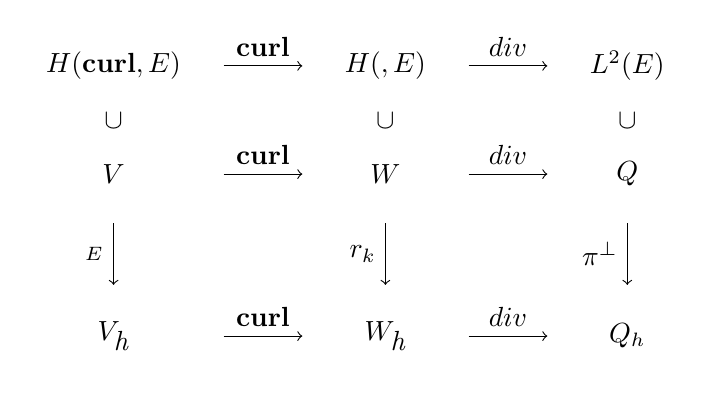
\begin{tikzpicture}[point/.style={circle, inner sep=0pt, minimum size=2pt,fill=red}]
            \matrix[column sep = 1.82mm, row sep = 1.1mm, ampersand replacement = \&] {
             \node {$\text{H}(\textbf{curl},E)$};  
              \& \node (n0) {};
              \& \node      {};
              \& \node (n1) {};
              \& \node (n2) {};
              \& \node {$\text{H}(\Div, E)$}; 
              \& \node (r1c7) {};
              \& \node {};
              \& \node {};
              \& \node (r1c10) {};
              \& \node {$L^2(E)$};\\
             \node (n3) {}; \&\&\&\&\& \node (n5)   {};
              \& \node (r2c7) {};
              \& \node {};
              \& \node {};
              \& \node {};
              \& \node (r2c11) {};\\
             \node (n4) {}; \&\&\&\&\& \node (n6)   {};
              \& \node (r3c7) {};
              \& \node {};
              \& \node {};
              \& \node {};
              \& \node (r3c11) {};\\
             \node (v)  {$V$}; \&\node(fromV){};\&\&\&\node(toW){};\& \node (w) {$W$};
              \& \node (r4c7) {};
              \& \node {};
              \& \node {};
              \& \node (r4c10) {};
              \& \node {$Q$};\\
             \node (n7) {}; \&\&\&\&\& \node (n8)   {};
              \& \node {};
              \& \node {};
              \& \node {};
              \& \node {};
              \& \node (r5c11) {};\\
             \node      {}; \&\&\&\&\& \node        {}; 
              \& \node {};
              \& \node {};
              \& \node {};
              \& \node {};
              \& \node {};\\
             \node      {}; \&\&\&\&\& \node        {}; 
              \& \node {};
              \& \node {};
              \& \node {};
              \& \node {};
              \& \node {};\\
             \node (n11)    {}; \&\&\&\&\& \node (n12) {};
              \& \node {};
              \& \node {};
              \& \node {};
              \& \node {};
              \& \node (r8c11) {};\\
             \node {$V_{\textit{h}} $};                                 
              \& \node (n13) {};
              \& \node       {};
              \& \node (n14) {};
              \& \node (n15) {};
              \& \node {$W_{\textit{h}} $}; 
              \& \node (r9c7) {};
              \& \node {};
              \& \node {};
              \& \node (r9c10) {};
              \& \node {$Q_h$};\\
             };
            \draw[->] (n0) to node[above] {$\textbf{curl}$} (n2); 
            \draw[->] (fromV) to node[above] {$\textbf{curl}$} (toW); 
            \draw[white] (n3) to node {{\color{black}$\cup$}} (n4);
            \draw[white] (n5) to node {{\color{black}$\cup$}} (n6);
            \draw[->] (n7) to node[left] {$\bw_E$} (n11); 
            \draw[->] (n8) to node[left] {$\boldsymbol{r}_k$} (n12); 
            \draw[->] (n13) to node[above] {$\textbf{curl}$} (n15); 
            \draw[->] (r1c7) to node[above] {$\text{div}$} (r1c10);
            \draw[->] (r4c7) to node[above] {$\text{div}$} (r4c10);
            \draw[->] (r9c7) to node[above] {$\text{div}$} (r9c10);
            %\draw[white] (r2c7) to node {{\color{black}$\cup$}} (r3c7);
            \draw[white] (r2c11) to node {{\color{black}$\cup$}} (r3c11);
            \draw[->] (r5c11) to node[left] {$\pi^{\perp}$} (r8c11);
        \end{tikzpicture}
    \end{center}
\begin{equation}\label{push-forward}
  \mbox{\color{red} \ldots \mbox{push-forward} de los interpoladores\\
    y que los pull--backs conmutan con los interpoladores}
\end{equation}
{\bf hcurl}
  
\begin{lemma} \label{aux_label7}
Let $\hat E$ be the reference prism~(\ref{defi_of_ref_prism}) and
let $P_{\hat E}$ be the space in~(\ref{spaceFEprismHcurl}), that is,
\begin{IEEEeqnarray*}{rCl}
  P_{\hat{E}} & = & R_k(\hat{x}_1,\hat{x}_2) \otimes P_k(\hat{x}_3) \times 
            P_k(\hat{x}_1,\hat{x}_2) \otimes P_{k-1}(\hat{x}_3).
\end{IEEEeqnarray*}
Provided the matrix $M_E$ is block--diagonal in this manner
\begin{IEEEeqnarray*}{rCl}
  M_E & = & \blockdiag{m_{1,1}}{m_{1,2}}{m_{2,1}}{m_{2,2}}{m_{3,3}}\mbox{,}
\end{IEEEeqnarray*}
then $P_{\hat{E}}$ is invariant by transformation~(\ref{transfHcurl}).
\end{lemma}
\begin{proof}
  Starting with transformation~(\ref{transfHcurl}) take 
  $\hat{\bu}=(\hat u_1,\hat u_2,\hat u_3)'\in P_{\hat E}$
  and $\bu := (M_E^{-t}\hat{\bu})\circ F_E^{-1}$.
  Let 
  \[
    M_2 = \left(
    \begin{array}{cc}
      m_{1,1}  & m_{1,2}\\
      m_{2,1}  & m_{2,2} 
    \end{array}
    \right)
  \]
  and let $m_{i,j}^{(-1)}$ denote the coefficients of the inverse.
  By definition, 
  $(\hat u_1,\hat u_2)' = \hat{q}(\hat\bp + \hat{\boldsymbol{s}})$ for some
  $\hat\bp$, $\hat{\boldsymbol{s}}$ as in~(\ref{defSk}) and~(\ref{defRk}) and
  $\hat{q}\in P_{k}(\hat x_3).$ Using the blocks of $M_E$ and the tensor nature of
  $P_{\hat E}$,
  \begin{IEEEeqnarray*}{rCl}
    (\hat u_1(\bx),\hat u_2(\bx))' & = & (\hat{q}M_2^{-t}(\hat\bp + 
      \hat{\boldsymbol{s}}))(M_E^{-1}\bx - M_E^{-1}\bx_E)\\
    & = & \hat{q}(m_{3,3}^{(-1)}(x_3-x_{E,3}))(M_2^{-t}(\hat\bp + 
      \hat{\boldsymbol{s}}))(M_2^{-1}\bx - M_2^{-1}\bx_E).
  \end{IEEEeqnarray*}
  Now, $\hat{q}(m_{3,3}^{(-1)}(x_3-x_{E,3}))$ is a polynomial $q(x_3)$ with the
  same 
  degree as $\hat{q}$ is qith respect to $\hat x_3$. Furthermore,
  as by Remark~(\ref{aux_label6}) $\hat{\boldsymbol{s}}$ has degree $\leqslant k-1$,
  $(M_2^{-t}(\hat\bp + \hat{\boldsymbol{s}}))(M_2^{-1}\bx - M_2^{-1}\bx_E)$
  can be seen as
  $M_2^{-t}(\bp(x_1,x_2) + \hat{\boldsymbol{s}}(M_2^{-1}\bx))$ with $\bp$
  having the expected degrees. And now
  \begin{IEEEeqnarray*}{rCcCl}
    M_2^{-t}\hat{\boldsymbol{s}}(M_2^{-1}\bx)\cdot(x_1,x_2)'
        &=& 
    \hat{\boldsymbol{s}}(M_2^{-1}(x_1,x_2)')\cdot M_2^{-1}(x_1,x_2)' &=& 0.
  \end{IEEEeqnarray*}
  The invariance of the third component of elements in $P_{\hat E}$ is
  an immediate consequence of the affine nature of the coordinate change.
\end{proof}
%=======================================================================
%\begin{remark} this is not a restriccion...
%  \begin{figure}
%    \centering
%    *** ***
%    \caption{hybrid mesh}\label{obliquePrism}
%  \end{figure}
%  dibujo prisma oblicuo subdividido: tetra + prism + pyramid. Figure~\ref{obliquePrism}
%\end{remark}
%=======================================================================
\begin{lemma} Let a physical prism $E = F_E(\hat{E})$ for $F_E$ as in~(\ref{aux_label8}).
Given $\hat\bu$ defined in $\hat{E}$ let $\bu$ in $E$ dtermined by~(\ref{transfHcurl}), and
let $\hat\btau$, $\btau$, $\hat\bnu$ and $\bnu$ be tangents and normals in
$\hat E$ and $E$ related by~(\ref{aux_label10}) and~(\ref{aux_label9}). Suppose
we define degrees of freedom of $\bu$ on $E$ as
\begin{IEEEeqnarray}{ll}
    \label{momentos1hcurlPhys}  
    \varphi_{\be_i,p}\,(\bu) = 
    \int_{\be} \bu \cdot \boldsymbol{\tau} \,q\, ds  
        & q\in P_{k-1}\mbox{,} \\
    \IEEEeqnarraymulticol{2}{l}{\nonumber\mbox{ for each edge $\be$ with unit tangent } \boldsymbol{\tau} \mbox{;}}\\[8pt]
    \label{momentos2hcurlPhys} 
    \varphi_{f,\bq}\,(\bu) =  
    \int_{f} \bu \cdot \bq_0\,
    dS\mbox{, } &\bq_0 = (\det M_E\|M_E^{-t}\hat\bnu\|)^{-1} M_E\hat{\bq}_T\\
    &\hat{\bq}_T := (\hat\bnu\times\hat\bq)\times\hat\bnu\\
    &\mbox{$\hat\bq$ as in~(\ref{momentos2hcurl})--(\ref{momentos5hcurl})}.\\[8pt]
    \label{momentos6hcurlPhys}
    \varphi_{\br}(\bu) = 
    \int_{E} \bu \cdot \br \, d\bx\mbox{, }&\br = (\det M_E)^{-1} M_E\hat\br \circ F_E^{-1}\\
    &{\nonumber\hat\br \in P_{k-2,k-2} \times P_{k-3,k-1}.}
\end{IEEEeqnarray}
Provided $\det > 0$, the degrees of freedom are identical
\end{lemma}
\begin{proof}
  Edge dofs: ver foto
  Take a param $\hat{\boldsymbol{\alpha}}(t):I=[0,1]\to \hat\be$ such that
  $\hat\btau=\stackrel{.}{\hat{\boldsymbol{\alpha}}}(t)/\|\stackrel{.}{\hat{\boldsymbol{\alpha}}}(t)\|$.
  As  a jacobian maps tangents into tangents,
  $\boldsymbol{\alpha}(t)=M_E{\hat\bx}(t) + \bx_E$ parameterizes
  $\be$. Then\\
  Edge dofs:
  \begin{IEEEeqnarray*}{rCl}
    \int_{\be}(q\bu)\cdot d\boldsymbol{\alpha}
    &=&\int_{I}
    q\bu(F\hat\bx(t)))\cdot M_E
    \stackrel{.}{\hat{\boldsymbol{\bx}}}(t)dt  \\[5pt]
    &=&\int_{I}
    \hat q(\hat\bx(t)) M_E^{-t}
    \hat\bu(\hat\bx(t))\cdot M_E\stackrel{.}{\hat{\boldsymbol{\bx}}}(t)dt\\[5pt]
    &=&\int_{\hat\be}(\hat q\hat\bu)\cdot d\boldsymbol{\hat\alpha}.
  \end{IEEEeqnarray*}
  Face dofs: 
  \begin{IEEEeqnarray*}{rCl}
    \int_{\hat f} \hat\bv\times\hat\bnu\cdot\hat\bq\times\hat\bnu\,d\hat S 
    & = & \int_{\hat f} (\hat\bnu\times\hat\bq)\times\hat\bnu\cdot\hat\bu\,d\hat S \\
    & = & \int_{\hat f} \det M_E\|M_E^{-t}\hat\bnu\| \bq_0 (F\hat\bx) \cdot \bu(F\hat \bx) d\hat S \\
    & = & \int_{ f} \bq_0 (\bx) \cdot \bu( \bx) d S
  \end{IEEEeqnarray*}
  Vol dofs:
  \begin{IEEEeqnarray}{rCl}
    \int_{E}\bv\cdot\br\,d\bx
    & = & 
    \int_{\hat E}M_E^{-t}\hat\bv(F_E^{-1}\bx)\cdot
      (\det M_E)^{-1}M_E\hat\br(F_E^{-1}\bx)\,d\hat\bx.\\
    & = & 
    \int_{\hat E}\hat\bv(\hat\bx)\cdot\hat\br(\hat\bx)\,d\hat\bx.
  \end{IEEEeqnarray} 
\end{proof}

\begin{lemma} The finite element in Definition~\ref{edgeelement}  is conforming
in $H\curl$ and unisolvent.
  theorem 8 page 75 in~\cite{nedelec2} is incomplete, because it is only on
  the reference element.
\end{lemma}

\begin{lemma} >Provided $\det M^{t} > 0$?, the edge element interpolators satisfy
\begin{IEEEeqnarray}{rCl}\label{piTransformado}
    \wku(\hat{\bx}) & = & M^{t} \bw_E\bu(F_E(\hat{\bx}))
\end{IEEEeqnarray}
That is, the interpolator commutes with the coordinate change~(\ref{transfHcurl}).
\end{lemma}
\begin{proof} 
\end{proof}

{\bf hcurl end}

{\bf hdiv begin}

\begin{lemma}\label{aux_label13} Let $\hat E$ be the reference prism~(\ref{defi_of_ref_prism}) and
let $P_{\hat E}$ be the space in~(\ref{prismaticSpace}).
Provided the matrix $M_E$ is block--diagonal as in Lemma~\ref{aux_label7},
then $P_{\hat{E}}$ is invariant by transformation~(\ref{transfDiv}).
\end{lemma}
\begin{proof} The proof uses the same straightforward approach as the proof of 
Lemma~\ref{aux_label7} and in a much simpler case. \noindent{\color{BrickRed}pensar esto}   
\end{proof}

\begin{lemma} \label{aux_label12}
The degrees of freedom are identical, surface and volumen integrals:
in which the faces are related by $F\hat{f} = f$.
\begin{IEEEeqnarray}{cCccl}
    \label{momentos1hdivPhys} 
    \rho_{ f,q}(\bv) & = & \int_{f} (\bv\cdot\bnu)q\,dS 
        &\quad & \mbox{for } q = \hat{q}\circ F_E^-1, \hat{q} \in P_{k-1}(\hat{f})\mbox{,}\\
    \nonumber&&&\quad&\mbox{if $ \hat{f} =  \hat{f}_3$ or $ \hat{f}_4$;}\\[5pt]
    \label{momentos2hdivPhys}
    \rho_{ f,q}(\bv) & = & \int_{f} (\bv\cdot\bnu)q\,dS 
        &\quad & \mbox{for } q = \hat{q}\circ F_E^-1, \hat{q} \in Q_{k-1, k-1}(\hat f)\mbox{,}\\
    \nonumber&&&\quad&\mbox{ if $ \hat{f} =  \hat{f}_1$, $ \hat{f}_2$ or $ \hat{f}_5$;}\\[5pt]
    \label{momentos3hdivPhys}
    \rho_{ \br}(\bv) & = & \int_{{E}} \bv\cdot\br\,d\bx 
        &\quad& \mbox{for }\br = M_E^{-t}\hat\br\circ F_E^{-1}, \hat\br\in (P_{k-2,k-1})^2 \times P_{k-1,k-2};
\end{IEEEeqnarray}
\end{lemma}
\begin{proof}
  Face dofs, by~(\ref{transfDiv}) and~(\ref{surface_diffs})
  Vol dofs
  \begin{IEEEeqnarray}{rCcCl}
    \int_{E}\bv\cdot\br\,d\bx
    & = & 
    \int_{\hat E}M_E\hat\bv\cdot M_E^{-t}\hat\br\,d\hat\bx.
    & = & 
    \int_{\hat E}\hat\bv\cdot\hat\br\,d\hat\bx.
  \end{IEEEeqnarray}
\end{proof}

\begin{lemma}
  If $\bu\in P_{E}$ is such that all the
  dofs~(\ref{momentos1hdivPhys}) or~(\ref{momentos2hdivPhys}) vanish
  on the respective face $f$, then the normal component of $\bu$ 
  vanishes identically on $f$.
\end{lemma}
\begin{proof}
  This fact is stated in the proof of Theorem 4, page $66$ of~\cite{nedelec2} 
  only for the reference prism. By transforming the degrees of freedom to 
  the faces of $\hat E$ and back to the faces of $E$ using Lemma~\ref{aux_label12}
  we get the result.
\end{proof}
\begin{lemma}
  If $\bu\in P_{E}$ is such that all the
  dofs~(\ref{momentos1hdivPhys})--(\ref{momentos3hdivPhys}) vanish, 
  then $\bu$ vanishes identically on $E$.
\end{lemma}
\begin{proof}
  In the case of the reference prism $\hat E$, we refer to the proof of 
  Theorem 4 in page $66$ of~\cite{nedelec2}.
  by the invariance of the finite element space under
  the change~(\ref{transfDiv}) (Lemma~\ref{aux_label13}) we have our result.
\end{proof}
\begin{corollary}
  Finite Element on $E$ is $H(\dv)$--conforming and unisolvent.
\end{corollary}
\begin{corollary}
  For any $\bv\in W^{1,1}(E)$ expressions 
  ~(\ref{momentos1hdivPhys})--(\ref{momentos3hdivPhys}) 
  determine a well defined local interpolate
  $\br_E\,\bu$ defined as the unique finite element function in $P_E$ such that
  \begin{IEEEeqnarray}{lClc}
    \rho_{f,\bq}\,(\bv - \br_E\,\bu) & = & 0 &
    \quad\mbox{for $\rho_{f,\bq}$ as in~(\ref{momentos1hdivPhys})
      and~(\ref{momentos2hdivPhys})}\\
    \rho_{\br}\,(\bv - \br_E\,\bu) & = & 0 &
    \quad\mbox{for $\rho_{\br}$ as in~(\ref{momentos3hdivPhys})}.
  \end{IEEEeqnarray}
\end{corollary}
And the momentos3hdivPhyswt important
\begin{corollary}
  Given $\bu \in W^{1,1}(E)$, then
  \begin{IEEEeqnarray}{rCl} \label{div_interp_commutes}
    \rku & = & \det M_E\,(M_E^{-1}\,\br_E\,\bu)\circ F_E\mbox{,}
  \end{IEEEeqnarray}
  that is, the $H(\dv)$ interpolator commutes with the coordinate
  change~(\ref{transfDiv}).
\end{corollary}

{\bf hdiv end}


\begin{remark}
  Unisolvence and conformity of the finite elements on tetrahedra in
  Section~\ref{sec:tetrahedralFEs}
  is proved in~\cite{monk}, Sections 5.4 and 5.5.
\end{remark}
%===========================
% See Lemmas 5.32 and 5.34 in pages 130 and 131 of~\cite{monk}, where
% it is proved for tetrahedra. Exacly the same considerations about the degrees
% of freedom therein apply to prove the Lemma for prisms or pyramids.  
% Ver (3.79) (3.80) en monk: transf. de normales y tangentes.\\\\
%===========================